%!TEX root = ../dokumentation.tex

%TODO: Einleitung überarbeiten
\chapter{Implementierung}\label{cha:Implementierung}
\section{Datenbank, Login und Registrierung}\label{Datenbank}
Zu Beginn verbindet sich der Server mit der Datenbank. Server und Datenbank können über einen vorher definierten Port kommunizieren. Der Server kann mittels Datenbankabfragen auf die gespeicherten Daten zugreifen. Wenn sich ein neuer User registriert, sendet der Client dem Server den Usernamen und das Passwort. Der Server fordert nun von der Datenbank alle gespeicherte Daten an, die mit dem Usernamen und dem Passwort übereinstimmen und entscheidet anhand dessen, ob der Username und das Passwort bereits vergeben sind oder noch frei sind. Wenn die Antwort der Datenbank ein leeres Objekt ist, ist noch kein User mit dem Usernamen und dem Passwort registriert und in der Datenbank wird ein neuer Eintrag erstellt. 
In der folgenden Abbildung \ref{fig:login} ist der Login-Prozess schematisch dargestellt.
\begin{figure}[H]
\centering
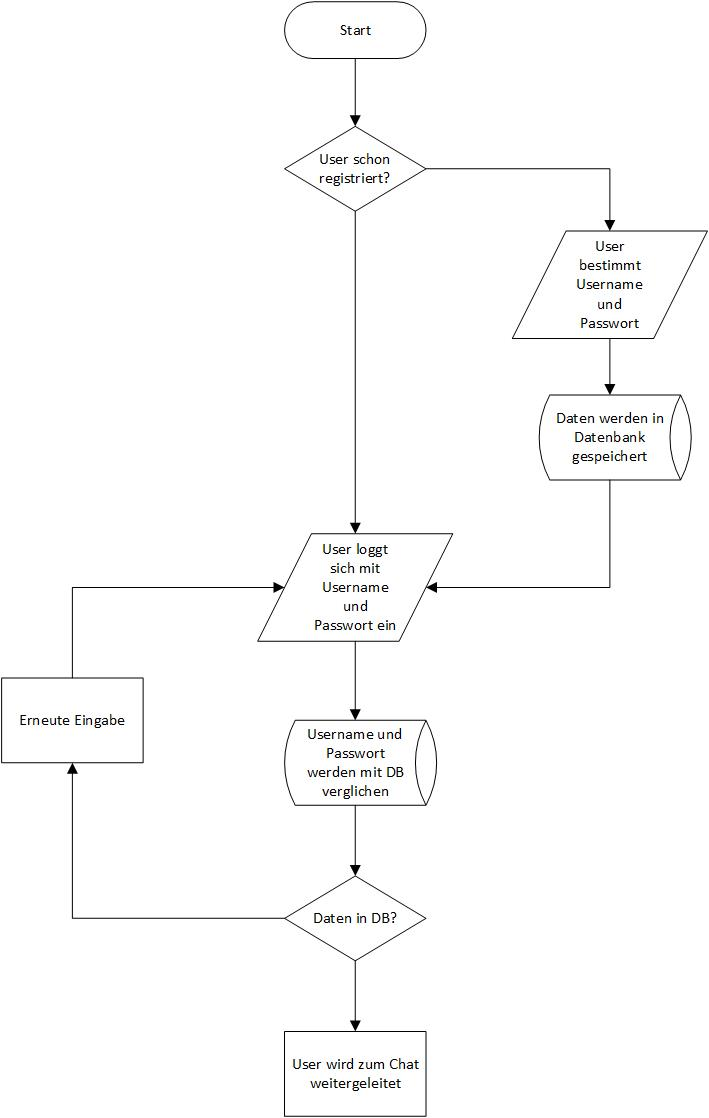
\includegraphics[width=0.7\textwidth]{images/login.jpg}
\caption{Flussdiagramm des Loginprozesses}
\label{fig:login}
\end{figure}

In folgenden Listing \ref{lis:mongodb} ist der Verbindungsaufbau mit der MongoDB gezeigt. In der URL ist die Portnummer des MongoDB-Container, über den die Verbindung aufgebaut wird, enthalten. Der darauffolgende Name ist der Name des Docker-Containers, aus dem die Datenbank aufgerufen wird.
In der letzten Zeile wird auf das definierte Datenbankschema verwiesen. 

\begin{lstlisting}[language=bash, caption={Verbindungsaufbau mit der MongoDB}, label=lis:mongodb]
mongoose
  .connect(
    'mongodb://mongo:27017/docker-node-mongo',
    { useNewUrlParser: true }
  )
  .then(() => console.log('MongoDB Connected'))
  .catch(err => console.log(err));

const User = require('./js/user');
\end{lstlisting}

In Listing \ref{lis:mongodbSchema} ist das Datenschema der Daten definiert, die in der MongoDB gespeichert werden. Die User-Informationen bestehen in dieser Anwendung aus einem Nutzernamen und einem Passwort. Beides wird benötigt und darf nicht leer bleiben. Außerdem sind beide vom Datentyp String.
\begin{lstlisting}[language=bash, caption={Datenschema in der MongoDB}, label=lis:mongodbSchema]
const mongoose = require('mongoose');
const Schema = mongoose.Schema;

const UserSchema = new Schema({
  name: {
    type: String,
    required: true
  },
  password: {
    type: String,
    required:true
  }
});

module.exports = User = mongoose.model('User', UserSchema);
\end{lstlisting}
\section{Spiellogik}\label{sec:Spiellogik}
Der User kann das Spiel über einen Knopf starten. Nun muss er warten bis ein anderer User das Spiel ebenfalls startet. Danach kann der User, der momentan an der Reihe ist, anhand von Knöpfen überhalb des Spielfeldes wählen, in welche Spalte er setzen möchte. Falls das Setzen nicht möglich ist, weil die Reihe schon voll ist, wird er zum erneuten Setzen an einer anderen Stelle aufgefordert. Wenn ein Spieler einen Stein setzen möchte, obwohl er nicht an der Reihe ist, wird diese Operation nicht durchgeführt. Nach jedem Zug wird geprüft, ob das Spiel vorbei ist. Wenn dies der Fall ist, kann ein neues Spiel begonnen werden. Dieser Ablauf ist in Abbildung \ref{fig:spiellogik} im Folgenden schematisch dargestellt.
\begin{figure}[H]
\centering
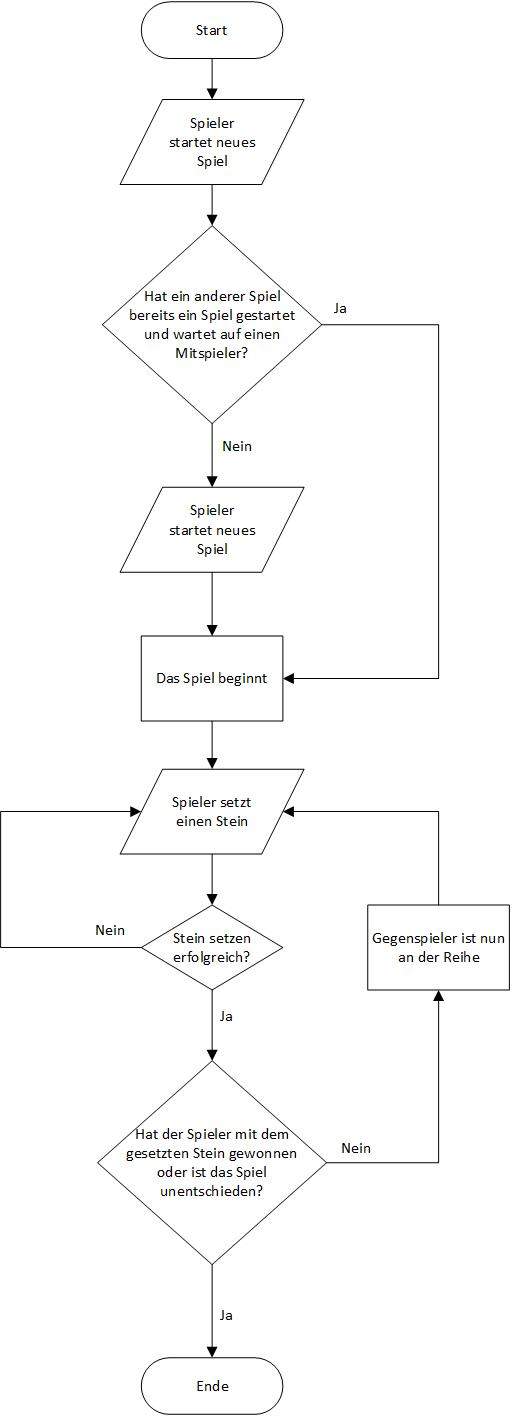
\includegraphics[width=0.5\textwidth]{images/spiellogik.jpg}
\caption{Flussdiagramm des Spielablaufs}
\label{fig:spiellogik}
\end{figure}

\section{Erkennung des Spielendes}\label{sec:GameOver}
Es gibt zwei Szenarien, unter denen das Spiel zu Ende ist. Entweder gewinnt ein Spieler oder das Spiel endet unentschieden. Unentschieden ist das Spiel, wenn das Spielfeld komplett gefüllt ist, aber kein Spieler eine Reihe aus vier Steinen aufbauen konnte.\\
Bei einem Gewinn sind drei verschiedene Szenarien zu unterscheiden. Eine Reihe aus vier Spielsteinen des gleichen Spielers kann horizontal, vertikal oder diagonal auftreten. Wenn die Reihe diagonal gebildet wird, kann noch zwischen von links unten nach rechts oben und von rechts unten nach links oben unterschieden werden. Alle diese Fälle müssen geprüft werden. Für jeden dieser Fälle hat der Server eine Funktion, um das Spielfeld zu überprüfen.\\
Als Beispiel wird im Folgenden in Listing \ref{lis:game_over_check} die Erkennung einer vertikalen Reihe aus vier Spielsteinen des gleichen Spielers erläutert. Wenn kein Spieler vertikal gewonnen hat, gibt diese Funktion den Wert $0$ zurück, ansonsten die ID des Spielers, der vertikal gewonnen hat. Dazu werden zwei verschachtelte For-Schleifen verwendet, wobei die äußere die Spalten des Spielfelds durchläuft und die innere ein Offset in den Zeilen erzeugt (Zeile 2 und 3). Die boolsche Variable $flag$, die in Zeile 4 deklariert und mit $true$ initialisiert wird, gibt an, ob im aktuellen Durchlauf ein Gewinner gefunden werden konnte. Ist $flag$ bei der if-Abfrage in Zeile 14 immer noch wahr, so wurde ein Gewinner gefunden. Dieser wird dann zurückgegeben. Hat der Spielstein ($lowestPlayerTile$) bei dem die Prüfung jeweils anfängt den Wert $0$, so muss nicht weiter geprüft werden, da dieses Feld noch von keinem Spieler besetzt wurde. Ist dies nicht der Fall, so wird die For-Schleife in Zeile 7 durchlaufen. Ausgehend von dem Spielstein $lowestPlayerTile$ werden dort die drei rechts davon liegenden Spielsteine überprüft. Ist einer davon nicht von dem selben Spieler wie $lowestPlayerTile$, so wird die Schleife abgebrochen und $flag$ auf falsch gesetzt, da dann kein Gewinn vorliegt. Gehören alle vier Spielsteine dem gleichen Spieler, so liegt ein Gewinn vor und die ID des Spielers wird zurückgegeben.
\begin{lstlisting}[language=bash, caption={Vertikale Game-Over Überprüfung}, label=lis:game_over_check]
function checkVerticalGameOver(game){
for (let column=0; column<7; column++){
  for (let row=0; row<3; row++) {
   var flag = true;
   var lowestPlayerTile = this._gameManager[game][0][row)[column];
     if (lowestPlayerTile != 0){
      for (let i=1; i<4; i++){
	     if(lowestPlayerTile !=
	      this._gameManager[game][0][row+1][column]){
	      flag = false;
	      break;
         }
      }
     if(flag == true){
      return lowestPlayerTile;
     }
    }
   }
  }
return 0;
}
\end{lstlisting}
\section{Docker Compose}\label{sec:Docker-Compose}
In einem Docker-Compose-File sind die zu verwaltenen Container mit den Portnummern, über die auf die Container zugegriffen werden kann, enthalten. In Listing \ref{lis:dockercompose} ist das Docker-Compose-File dieser Anwendung dargestellt. In der ersten Zeile wird das Docker-Compose-File-Format genannt. Version 3 ist die aktuelle Version. In den folgenden Zeilen werden die einzelnen Services, also die einzelnen Docker-Container festgelegt. Der Container-Name in Zeile 4 beschreibt den Namen des Docker-Containers, der anstatt eines automatisch festgelegtem Namen benutzt wird. In Zeile 6 wird der Pfad hinterlegt, in dem das Docker-File hinterlegt ist, welches die build-Funktion spezifiziert. $Links$ in Zeile 10 benennt Links zu anderen Containern, in diesem Fall zu dem MongoDB-Container. Die Portnummern beschreiben die Abbildung von Container-internen auf externe Portnummern. Mit Hilfe der externen Portnummer können die Docker-Container miteinander kommunizieren, bzw. kann mit den Docker-Containern von außen kommuniziert werden. In Zeile 14 ist der Name des erstellten Images festgelegt, aus dem der Container gestartet wird.
\newpage
\begin{lstlisting}[language=bash, caption={docker-compose.yml-File}, label=lis:dockercompose]
version: '3'
services:
  app:
    container_name: docker-node-mongo
    restart: always
    build: .
    ports:
      - '80:3000'
      - '8181:8181'
    links:
      - mongo
  mongo:
    container_name: mongo
    image: mongo
    ports:
      - '27017:27017'


\end{lstlisting}


